\section{Compressed Histogram of Gradients descriptor}

\subsection{Patch extraction and normalization}

Once points of interest have been selected at different scales, patches are formed. A patch is square area that has the point of interest at its center. The patch is at the same scale as the point of interest and its size depends on that scale \cite{Mikolajczyk2005PEL}. As is, this area of the image is susceptible to rotation and illumination changes. Therefore both the orientation and illumination are normalized.

The orientation of the patch matches the direction of the most pronounced gradient in the neighbourhood of the interest point (The local gradients are sorted in a histogram, each bin containing a gradient angle weighted by the gradient magnitude. The dominant gradient is selected by taking the largest bin.) \cite{Lowe04distinctiveimage}.

The mean and standard deviation of the pixel values of the patch are normalized in order to compensate for affine transformations in illumination ($aI(x) + b$) \cite{Mikolajczyk2005PEL}. Non linear changes in illumination cannot be easily modeled and compensated.

Chandrasekhar et al.\ \cite{chog2011} also apply Gaussian smoothing to the patch (with $\sigma = 2.7$ pixels).

\subsection{Spatial binning}

First of all, the patch is subdivided into cells arranged according to a DAISY configuration \cite{Tola08,best_daisy}. See figure~\ref{fig:daisy_regions} for an example with 9 spatial bins.

Overlapping bins are used to compensate for errors in the locations of the points of interest \cite{chog2011}. Soft assignment is used, i.e.\ each pixel contributes to more than one spatial bin. The closer a pixel is to the centroid of a bin, the less it contributes to neighbouring spatial bins. This is reflected by assigning a normalized Gaussian weight to each bin, the sum of all weights being 1. Chandrasekhar et al.\cite{chog2011} use $\sigma=d_{min}/3$ as a paramater to the Gaussian, where $d_{min}$ is the smallest distance between cell centroids in the DAISY configuration.

\begin{figure}
    \centering
    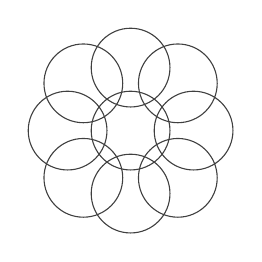
\begin{tikzpicture}
        \draw[darkgray] (0,0) circle (0.5);
        \draw[darkgray] (0,0.8) circle (0.5);
        \draw[darkgray] (0,-0.8) circle (0.5);
        \draw[darkgray] (0.8,0) circle (0.5);
        \draw[darkgray] (-0.8,0) circle (0.5);
        \draw[darkgray] (0.6,0.6) circle (0.5);
        \draw[darkgray] (-0.6,0.6) circle (0.5);
        \draw[darkgray] (0.6,-0.6) circle (0.5);
        \draw[darkgray] (-0.6,-0.6) circle (0.5);
    \end{tikzpicture}
    \caption{
        An approximation of a DAISY-9 configuration. Contrary to the configuration in \cite{best_daisy} which features disjoint cells, the regions used in \cite{chog2011} overlap, as depicted here.
        \label{fig:daisy_regions}
    }
\end{figure}


\subsection{Gradient histogram binning}

The image gradients with respect to $x$ and $y$ are computed with [-1 0 -1] as filter. The joint gradient ($d_x$, $d_y$) is put into bins by means of vector quantization. Different quantization configuration can be seen in figure~\ref{fig:voronoi_regions}. Chandrasekhar et al.\ \cite{chog2011} claim that statistical analysis of a large data set suggests bins should be positioned such that the bin centers are at even distances on an ellipse centered at $(0,0)$. Furthermore, there is a bin with center $(0,0)$ which is the most statistically significant point in the joint gradient distribution. As with spatial binning, the joint gradients are assigned to multiple bins with Gaussian weights. The Gaussian parameter is $\sigma = d_{min}/3$, where $d_{min}$ is the smallest distance between centroids.

Chandrasekhar et al.\ also evaluate and discuss the performance of the different bin layouts. A larger number of quantization cells yields a higher precision. An evaluation of feature descriptors in a common framework \cite{chog2011} shows that the uncompressed histogram of gradients with a DAISY-9 spatial binning configuration and a VQ-5 gradient histogram binning configuration outperforms the popular SIFT descriptor \cite{Lowe04distinctiveimage}.

\begin{figure}
    \centering
    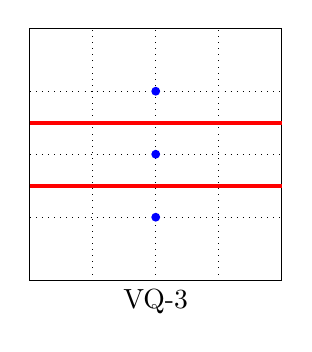
\begin{tikzpicture}[scale=0.8]
        \draw (-2,-2) rectangle (2,2);
        \draw[step=1, dotted, very thin] (-2,-2) grid (2,2);
        \fill[blue] (0,0) circle (2pt);
        \fill[blue] (0,1) circle (2pt);
        \fill[blue] (0,-1) circle (2pt);
        \draw[red,line width=1.5pt] (-2,0.5) -- (2,0.5);
        \draw[red,line width=1.5pt] (-2,-0.5) -- (2,-0.5);
        \draw (0,-2) node[below] {VQ-3};
    \end{tikzpicture}
    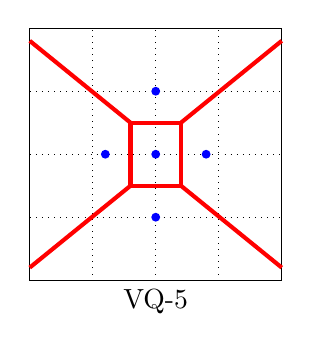
\begin{tikzpicture}[scale=0.8]
        \draw (-2,-2) rectangle (2,2);
        \draw[step=1, dotted, very thin] (-2,-2) grid (2,2);
        \fill[blue] (0,0) circle (2pt);
        \fill[blue] (0,1) circle (2pt);
        \fill[blue] (0,-1) circle (2pt);
        \fill[blue] (-0.8,0) circle (2pt);
        \fill[blue] (0.8,0) circle (2pt);
        \draw[red,line width=1.5pt] (-0.4,0.5) rectangle (0.4,-0.5);
        \draw[red,line width=1.5pt] (-2,1.8) -- (-0.4,0.5);
        \draw[red,line width=1.5pt] (-2,-1.8) -- (-0.4,-0.5);
        \draw[red,line width=1.5pt] (2,1.8) -- (0.4,0.5);
        \draw[red,line width=1.5pt] (2,-1.8) -- (0.4,-0.5);
        \draw (0,-2) node[below] {VQ-5};
    \end{tikzpicture}
    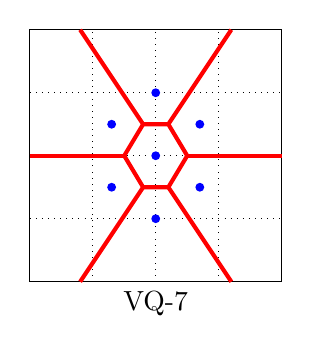
\begin{tikzpicture}[scale=0.8]
        \draw (-2,-2) rectangle (2,2);
        \draw[step=1, dotted, very thin] (-2,-2) grid (2,2);
        \fill[blue] (0,0) circle (2pt);
        \fill[blue] (0,1) circle (2pt);
        \fill[blue] (0,-1) circle (2pt);
        \fill[blue] (0.7,0.5) circle (2pt);
        \fill[blue] (0.7,-0.5) circle (2pt);
        \fill[blue] (-0.7,0.5) circle (2pt);
        \fill[blue] (-0.7,-0.5) circle (2pt);
        \draw[red,line width=1.5pt]
            (-0.5,0) coordinate (a) --
            (-0.2,0.5) coordinate (b) --
            (0.2,0.5) coordinate (c) --
            (0.5,0) coordinate (d) --
            (0.2,-0.5) coordinate (e) --
            (-0.2,-0.5) coordinate (f) -- (a);
        \draw[red,line width=1.5pt] (-2,0) -- (a);
        \draw[red,line width=1.5pt] (-1.2,2) -- (b);
        \draw[red,line width=1.5pt] (1.2,2) -- (c);
        \draw[red,line width=1.5pt] (2,0) -- (d);
        \draw[red,line width=1.5pt] (1.2,-2) -- (e);
        \draw[red,line width=1.5pt] (-1.2,-2) -- (f);
        \draw (0,-2) node[below] {VQ-7};
    \end{tikzpicture}
    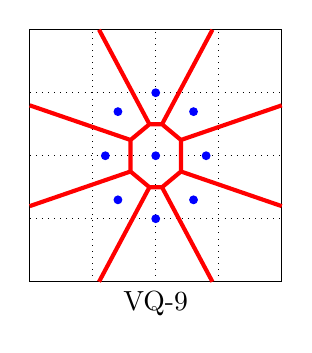
\begin{tikzpicture}[scale=0.8]
        \draw (-2,-2) rectangle (2,2);
        \draw[step=1, dotted, very thin] (-2,-2) grid (2,2);
        \fill[blue] (0,0) circle (2pt);
        \fill[blue] (0,1) circle (2pt);
        \fill[blue] (0,-1) circle (2pt);
        \fill[blue] (-0.8,0) circle (2pt);
        \fill[blue] (0.8,0) circle (2pt);
        \fill[blue] (0.6,0.7) circle (2pt);
        \fill[blue] (0.6,-0.7) circle (2pt);
        \fill[blue] (-0.6,0.7) circle (2pt);
        \fill[blue] (-0.6,-0.7) circle (2pt);
        \draw[red,line width=1.5pt]
            (-0.4,0.25) coordinate (a) --
            (-0.1,0.5) coordinate (b) --
            (0.1,0.5) coordinate (c) --
            (0.4,0.25) coordinate (d) --
            (0.4,-0.25) coordinate (e) --
            (0.1,-0.5) coordinate (f) --
            (-0.1,-0.5) coordinate (g) --
            (-0.4,-0.25) coordinate (h) -- (a);
        \draw[red,line width=1.5pt] (-2,0.8) -- (a);
        \draw[red,line width=1.5pt] (-0.9,2) -- (b);
        \draw[red,line width=1.5pt] (0.9,2) -- (c);
        \draw[red,line width=1.5pt] (2,0.8) -- (d);
        \draw[red,line width=1.5pt] (2,-0.8) -- (e);
        \draw[red,line width=1.5pt] (0.9,-2) -- (f);
        \draw[red,line width=1.5pt] (-0.9,-2) -- (g);
        \draw[red,line width=1.5pt] (-2,-0.8) -- (h);
        \draw (0,-2) node[below] {VQ-9};
    \end{tikzpicture}
    \caption{
        Voronoi cells for the histogram quantization. The dots represent the cell centroids. The naming comes from \cite{chog2011} and conveys the number of cells in each vector quantization configuration.
        \label{fig:voronoi_regions}
    }
\end{figure}


\subsection{Quantization and compression}

So far we have an uncompressed histogram of gradients. The next step is to compress the descriptor while aiming for fast and accurate matching.

The original paper on CHoG \cite{chog2009} used Huffman tree coding for quantization. The authors have since improved the descriptor by switching to type coding which has better time complexity \cite{chog2011}. Entropy Constrained Vector Quantization is optimal in terms of rate and distortion, but unpractical in the context of mobile search: it is more complex and requires storing codebooks on the device \cite{chog2011}.

\subsubsection{Latices}

\subsubsection{Type coding}
\label{sec:type_coding}

\subsubsection{Quantization}

Chandrasekhar et al.\ \cite{chog2011} use the following algorithm to quantize a distribution $P$ to the nearest type in $Q_n$ ($Q_n$ is as described in section~\ref{sec:type_coding})
\begin{enumerate}

\item With $i=1,\ldots,m$, compute: \begin{displaymath}
k_i^\prime = \lfloor np_i+\frac{1}{2} \rfloor,\quad n^\prime=\sum_i k_i^\prime
\end{displaymath}

\item \label{algo:step_sort} If $n^\prime = n$, the nearest type is given by the paramaters $k_i^\prime$. Return $k_i = k_i^\prime$. Otherwise, compute the errors
\begin{displaymath}
\delta_i = k_i^\prime - np_i
\end{displaymath}
 and sort them s.t.
\begin{displaymath}
-\frac{1}{2} \leq \delta_{j_1} \leq \delta_{j_2} \leq \cdots \leq \delta_{j_m} \leq \frac{1}{2}
\end{displaymath}

\item \label{algo:step_decrincr} Let $d = n^\prime - n$. If $d > 0$ then decrement $d$ values $k_i^\prime$ with largest errors.
\[
k_{j_i} = \begin{cases}
k_{j_i}^\prime & j = i,\ldots,m-d-1, \\
k_{j_i} & i=m-d,\ldots,m,
\end{cases}
\]
otherwise, if $d < 0$ increment $\left|d\right|$ values $k_i^\prime$ with smallest errors
\[
k_{j_i} = \begin{cases}
k_{j_i}^\prime + 1 & i = 1,\ldots,\left|d\right|, \\
k_{j_i} & i=\left|d\right|+1,\ldots,m.
\end{cases}
\]

\item Return $k_1,\ldots,k_m$.
\end{enumerate}

Because in step~\ref{algo:step_decrincr} only the $\left|d\right|$ smallest or largest elements are needed, a full sort of the errors $\delta_i$ in step~\ref{algo:step_sort} is unnecessary. Reznik et al.\ \cite{fastchog} show that $\left|d\right|$ is small in practice and propose to simply select the $\left|d\right|$ smallest/largest elements, thus reducing the overall complexity of the algorithm.

Reznik et al.\ also add a bias to the reconstruction points:
\begin{equation}
    q_i^\prime = \frac{k_i + \beta}{n + \beta m}, \quad i = 1,\ldots,m.
\end{equation}
with the bias parameter $\beta = \beta_0\frac{n}{n_0}$ where $n_0$ is the total number of samples in the non-quantized histogram and $\beta_0 = \frac{1}{2}$ as used in the computation of the probabilities:
\begin{equation}
    p_i^\prime = \frac{k_{0,i} + \beta_0}{n_0 + \beta_0 m}, \quad i = 1,\ldots,m.
\end{equation}

\subsubsection{Encoding}

The disired property of the encoding scheme is to eliminate the need of storing a codebook for encoding and decoding. Chandrasekhar et al.\ \cite{chog2011} use an enumeration method that allows the computation of index on the fly, based on the type parameters.

The number of types in lattice $Q_n$ is given by the number partitions of $n$ into $m$ terms $k_1 + \cdots  + k_m = n$ \cite{chog2011}:
\begin{equation}
\left|Q_n\right| = {n+m-1 \choose m-1}
\end{equation}

Let $\xi(k_1, \ldots k_m)$ be the index of the type with parameters $k_1, \ldots, k_m$. A lexicographic enumeration of the types is:
\begin{align*}
&\xi(0,0,\ldots,0,n) = 1 \\
&\xi(0,0,\ldots,1,n-1) = 2 \\
&\ldots \\
&\xi(n,0,\ldots,0,0) = {n+m-1 \choose m-1} - 1
\end{align*}
The generalized formula \cite{chog2011} is:
\begin{equation}
\xi(k_1, \ldots, k_m) = \sum_{j=1}^{m-2} \sum_{i=0}^{k_j - 1} {n-i-\sum_{l=1}^{j-1}k_l+m-j-1 \choose m-j-1} + k_{n-1}
\end{equation}

